\documentclass[11pt]{article}
\usepackage[utf8]{inputenc}
\usepackage[T1]{fontenc}
\usepackage{lmodern}
\usepackage{amsmath,amssymb}
\usepackage{float}
\usepackage[a4paper, margin=2.0cm, headheight=13pt]{geometry}
\usepackage{graphicx}
\graphicspath{{../../evaluation/results/2026-11-16/figures/}}
\usepackage{booktabs}
\usepackage{array}
\usepackage{tabularx}
\usepackage{longtable}
\usepackage{enumitem}
\usepackage{xcolor}
\usepackage{caption}
\usepackage{fancyhdr}
\usepackage{hyperref}
\hypersetup{colorlinks=true, linkcolor=black, urlcolor=blue!50!black,
  pdftitle={Experimental Evaluation and Results}, pdfauthor={Project 01, Group 33}}
\setlist{itemsep=1pt, topsep=3pt, leftmargin=1.3em}
\renewcommand{\arraystretch}{1.18}
\setlength{\parskip}{4pt}
\setlength{\parindent}{0pt}
\setlength{\emergencystretch}{3em}
\newcolumntype{L}{>{\raggedright\arraybackslash}X}
\newcolumntype{P}[1]{>{\raggedright\arraybackslash}p{#1}}
\captionsetup{font=small, labelfont=bf, skip=4pt}
\pagestyle{fancy}
\fancyhf{}
\fancyhead[L]{\small Experimental Evaluation and Results}
\fancyhead[R]{\small Project 01 \textperiodcentered{} Group 33 \textperiodcentered{} CS5903}
\fancyfoot[C]{\small\thepage}
\newcommand{\code}[1]{\texttt{\small #1}}
\newcommand{\repo}{https://github.com/krishnateja2314/iam-provider}
\newcommand{\gh}[2]{\href{\repo/blob/cs5903-final-2026/#1}{#2}}
\newcommand{\ghtree}[2]{\href{\repo/tree/cs5903-final-2026/#1}{#2}}
\makeatletter
\renewcommand\section{\@startsection{section}{1}{0pt}{-12pt plus -2pt}{5pt}{\large\bfseries}}
\renewcommand\subsection{\@startsection{subsection}{2}{0pt}{-8pt plus -2pt}{3pt}{\normalsize\bfseries}}
\makeatother

\begin{document}
\begin{center}
{\small Indian Institute of Technology Hyderabad \textperiodcentered{} CS5903 \textperiodcentered{} Final Project Submission}\\[6pt]
{\LARGE\bfseries Experimental Evaluation and Results}\\[4pt]
{\large Secure Multi-Tenant Identity and Access Platform}\\[6pt]
{\small Project 01 \textperiodcentered{} Group 33 \textperiodcentered{} Krishna Teja (CS23BTECH11028), Jaya Prakash (CS23BTECH11015)}\\
{\small Repository \url{\repo} \textperiodcentered{} tag \texttt{cs5903-final-2026} \textperiodcentered{} code revision \texttt{e13f019} \textperiodcentered{} 16 November 2026}
\end{center}

\section{Summary of evidence}
\begin{table}[H]
\centering\small
\begin{tabularx}{\textwidth}{@{}P{6.2cm} L@{}}
\toprule
\textbf{Claim} & \textbf{Evidence (expected $\rightarrow$ observed)}\\
\midrule
All frozen acceptance tests pass from a clean clone & 0 failed, 0 skipped $\rightarrow$ \textbf{253 passed, 0 failed, 0 skipped} (14 Nov, \texttt{e13f019}); repeated 16 Nov in a fresh clone of the submission: \textbf{253/253}\\
The tests can detect real security bugs & every injected bug caught $\rightarrow$ \textbf{15/15 mutations killed}; database stopped $\rightarrow$ \textsc{inconclusive} (exit 2), never ``success''\\
Revoked sessions/agents are refused on the next request, unlike the baseline & solution 401 on first request $\rightarrow$ \textbf{15/15}; baseline (JWT-only) $\rightarrow$ accepted \textbf{15/15}, agent tokens for a median \textbf{59.4\,s}\\
The real browser flow works on two host names & 11/11 $\rightarrow$ \textbf{11/11 on \code{localhost}, 11/11 on \code{127.0.0.1}}\\
AG02 agents never exceed their user & intersection holds $\rightarrow$ \textbf{26/26} AG02 tests, mutations M12--M15 killed\\
Price of the per-request check & observation $\rightarrow$ introspection p50 \textbf{3.3\,ms} of a \textbf{9.3\,ms} authenticated request\\
\bottomrule
\end{tabularx}
\caption{What this document shows. Every number names its revision and date; raw logs are linked in \S9.}
\end{table}

\section{Evaluation questions and metrics}
\begin{table}[H]
\centering\small
\begin{tabularx}{\textwidth}{@{}l L P{4.0cm} P{4.2cm}@{}}
\toprule
\textbf{ID} & \textbf{Question} & \textbf{Metric (unit)} & \textbf{Pass threshold (frozen 10 Oct)}\\
\midrule
Q1 & Do all acceptance tests pass from a clean clone? & tests passed/failed/skipped & 0 failed, 0 skipped\\
Q2 & Can the tests fail (do they catch real bugs)? & mutations killed / total & all killed; DB down $\Rightarrow$ exit 2\\
Q3 & Is a revoked credential refused on the next request, vs the baseline? & first-request status; seconds accepted; requests accepted afterwards & 401 first request, $\le$\,5000\,ms, 0 accepted afterwards\\
Q4 & What does the per-request check cost? & p50/p95 latency (ms) & observation only\\
Q5 & Does the real-browser flow hold on two hosts? & browser checks passed & 11/11 on both\\
Q6 & Does AG02 never exceed its user? & outcome table & as specified in ADR-014\\
\bottomrule
\end{tabularx}
\caption{Evaluation questions (\gh{docs/evaluation-protocol.md}{\code{docs/evaluation-protocol.md}}).}
\end{table}

\section{Setup}
\textbf{Hardware/software.} One laptop with Windows~11 Home and Docker Desktop (Linux containers). Images: \code{node:24.21.0-alpine}, \code{postgres:16.15-alpine}, \code{quay.io/keycloak/keycloak:26.8.0}. Dependencies are pinned by \code{backend/package-lock.json} (Fastify 5.12.8, Casbin 5.51.1, jose 6.2.12, Vitest 5.0.3). Browser: Microsoft Edge driven by Playwright 1.63.0.

\textbf{Data/workload.} Synthetic and committed in the repository: two Keycloak realms, three tenants, five users, courses and submissions. There are no external datasets and no personal data. There are no random seeds: fixtures use fixed UUIDs, and the per-trial users of experiment E1 (\code{eval-<uuid>}) do not affect any outcome.

\textbf{Baselines.}
\begin{itemize}
  \item \textbf{B0, JWT-only validation} (security baseline). Accept any access token whose RS256 signature, issuer, audience, expiry and \code{typ=Bearer} verify against the provider's keys, with no introspection. This is the common shortcut, and it is exactly the first half of our own validator. It runs against the same live tokens as our API.
  \item \textbf{Revision baseline.} The Week~3 head \texttt{953a0aa}, rerun on 31 Oct before any fix.
  \item \textbf{Guard-removed baselines.} Each mutation M1--M15 is our system with exactly one security guard removed.
\end{itemize}

\section{Experiment E1: baseline vs solution after revocation (Q3)}
\textbf{Procedure.} For each trial: create a fresh user (or take a fresh AG01 agent token), confirm that B0 accepts the token and the API returns 200, then apply one operation: provider logout, admin logout-all, AG01 client disabled at the provider, or \emph{password reset} as a control (not a revocation). Present the same token to B0 and to the API once immediately, and then every 1\,s until it expires. There were 5 trials per operation (20 in total). Script: \gh{evaluation/scripts/baseline-revocation.mjs}{\code{evaluation/scripts/baseline-revocation.mjs}}.

\begin{table}[H]
\centering\small
\begin{tabular}{@{}lcccccc@{}}
\toprule
 & \textbf{Valid} & \textbf{B0} & \textbf{Ours} & \textbf{Ours: ms} & \textbf{B0} & \textbf{Ours}\\
\textbf{Operation (5 trials)} & \textbf{before} & \textbf{1st req.} & \textbf{1st req.} & \textbf{to 401} & \textbf{after} & \textbf{after}\\
\midrule
Provider logout & 5/5 & accepted 5/5 & \textbf{401} 5/5 & 22 ms & 15 of 30 & \textbf{0}\\
Admin logout-all & 5/5 & accepted 5/5 & \textbf{401} 5/5 & 13 ms & 15 of 30 & \textbf{0}\\
AG01 client disabled & 5/5 & accepted 5/5 & \textbf{401} 5/5 & 7 ms & 298 of 313 & \textbf{0}\\
Password reset (control) & 5/5 & accepted 5/5 & accepted 5/5 & --- & 15 of 30 & 15 of 30\\
\bottomrule
\end{tabular}
\caption{E1 results, 16 Nov 2026 (development stack, code identical to \texttt{e13f019}). ``ms to 401'' is the median time from the operation to the first refused request; ``after'' counts requests accepted while polling until expiry. Raw: \gh{evaluation/results/2026-11-16/e1-baseline-revocation.jsonl}{\code{e1-baseline-revocation.jsonl}}, \gh{evaluation/results/2026-11-16/summary.csv}{\code{summary.csv}}.}
\end{table}

\begin{figure}[H]
\centering
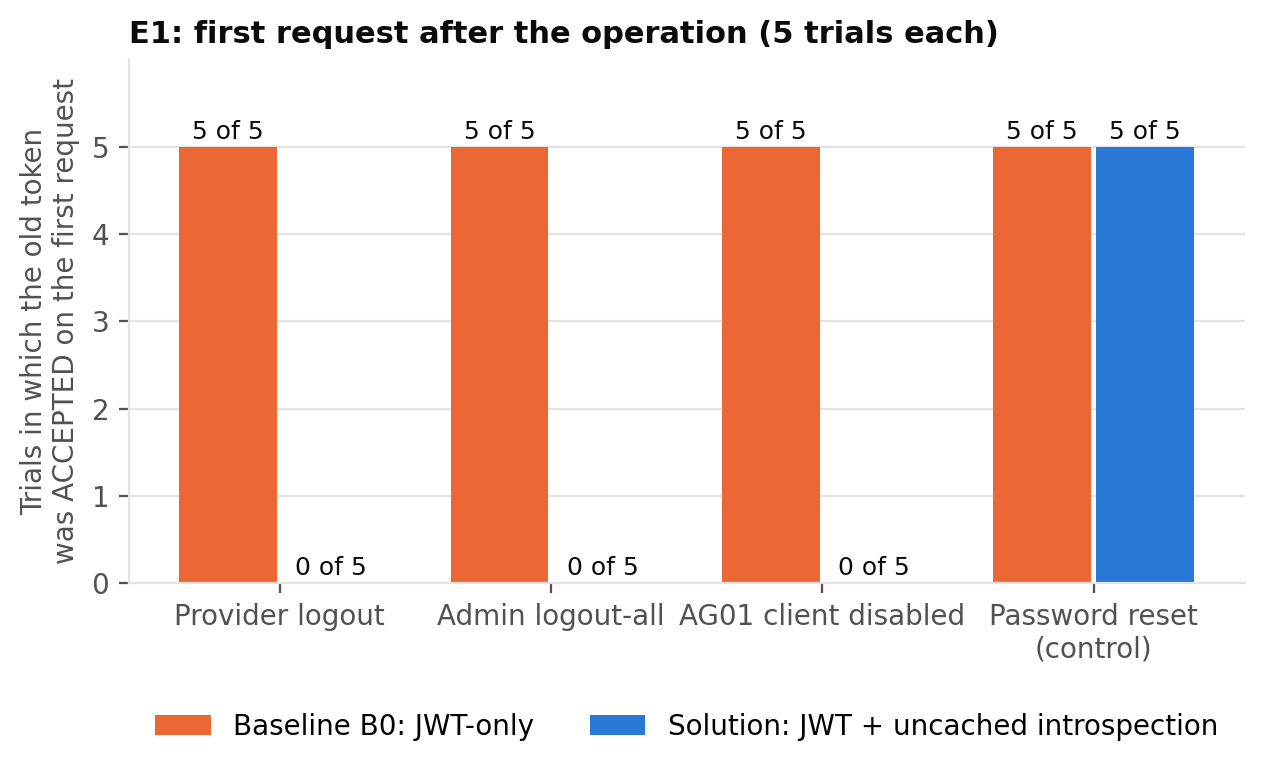
\includegraphics[width=0.49\textwidth]{e1-revoked-token-acceptance.png}\hfill
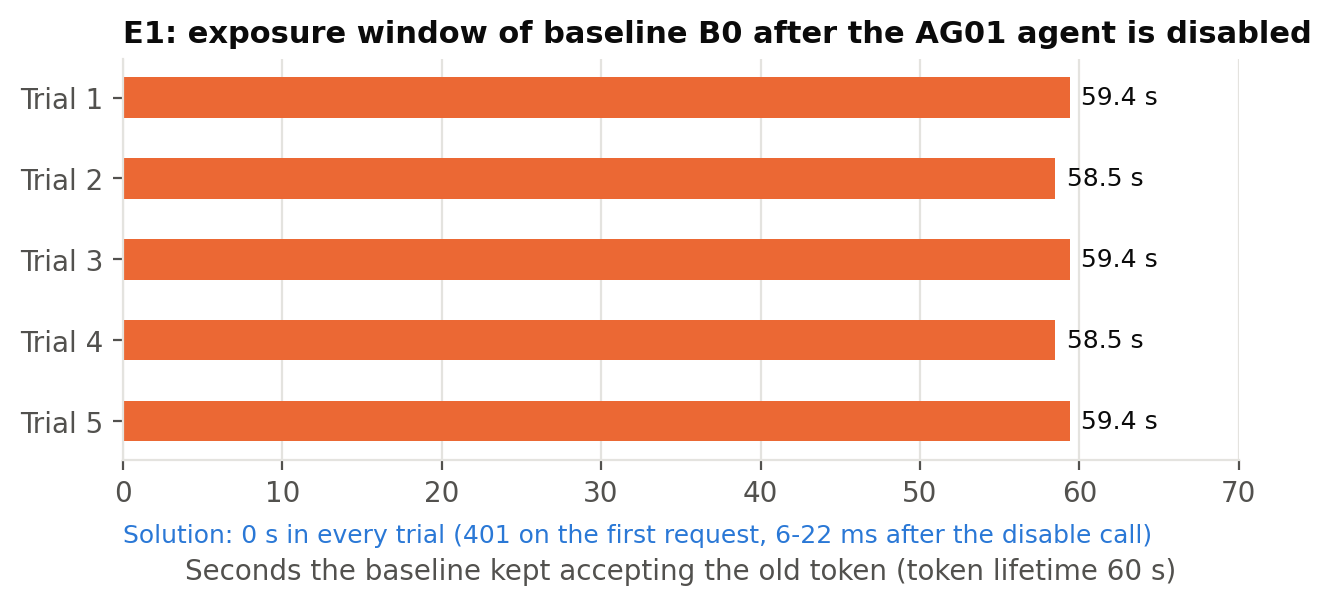
\includegraphics[width=0.49\textwidth]{e1-agent-exposure-window.png}
\caption{Left: trials in which the old token was still accepted on the first request after the operation. Right: how long B0 kept accepting a disabled agent's token (60\,s token lifetime); ours refused it immediately in every trial.}
\end{figure}

\begin{table}[H]
\centering\small
\resizebox{\textwidth}{!}{\begin{tabular}{@{}lccccc@{}}
\toprule
\textbf{AG01 trial} & 1 & 2 & 3 & 4 & 5\\
\midrule
B0 accepted (requests / polls) & 60/63 & 59/62 & 60/63 & 59/62 & 60/63\\
B0 exposure window (s) & 59.4 & 58.5 & 59.4 & 58.5 & 59.4\\
Ours: first request & 401 (22 ms) & 401 (7 ms) & 401 (8 ms) & 401 (6 ms) & 401 (6 ms)\\
Ours accepted afterwards & 0 & 0 & 0 & 0 & 0\\
\bottomrule
\end{tabular}}
\caption{Per-trial results for the agent scenario.}
\end{table}

\textbf{Reproduction in a clean clone.} The same experiment was repeated on 16 Nov in a fresh clone of the submission commit with new volumes. The verdicts were the same: B0 accepted 15/15 on the first request (agent median 58.6\,s); ours returned 401 on the first request in 15/15 trials (median 31 / 16 / 8\,ms) and accepted 0 afterwards (\ghtree{evaluation/results/2026-11-16-clean}{\code{2026-11-16-clean/}}).

\textbf{Observations.}
\begin{itemize}
  \item B0 cannot see revocation at all: it accepts a revoked token until \code{exp}. For agents that is the full 60\,s. For human web tokens (lifespan 300\,s) it would be up to five minutes.
  \item The human trials use the opt-in \code{iam-test} client, whose sessions end after 3\,s (it exists for expiry tests). That is why their polling stops after about 2\,s. The first-request result is unaffected.
  \item \textbf{Failure we disclose:} after a \emph{password reset}, neither B0 nor our API rejects the old token. Keycloak keeps existing sessions alive on reset. This is measured provider behaviour and is already recorded in the frozen protocol (criterion 3). Incident response must call logout-all.
\end{itemize}

\section{Complete test suite (Q1)}
\begin{table}[H]
\centering\small
\begin{tabular}{@{}lrrr@{}}
\toprule
\textbf{Test file} & \textbf{Passed} & \textbf{live Keycloak} & \textbf{Week 5}\\
\midrule
\code{t05-t08-authorization} (target: 40 scenarios) & 59 & --- & 59\\
\code{t03-t04-t09-token-validation} & 41 & --- & 41\\
\code{api} (integration, cross-tenant) & 31 & --- & 31\\
\code{service-principal} (AG01) & 30 & 7 & 30\\
\code{delegation} (AG02) & 26 & 4 & ---\\
\code{session-lifecycle} & 21 & 6 & 21\\
\code{startup-config} & 12 & --- & 12\\
\code{tenant-sso} & 10 & 3 & 10\\
\code{provisioning-privacy} & 9 & --- & 9\\
\code{t01-t02-identity-membership} & 8 & --- & 8\\
\code{t10-audit} & 6 & --- & 6\\
\midrule
\textbf{Total} & \textbf{253} & \textbf{20} & 227\\
\bottomrule
\end{tabular}
\caption{Final clean-clone run, 14 Nov 2026 (\texttt{e13f019}): 253 passed, 0 failed, 0 skipped, 11 files, 18.8\,s. Repeated 16 Nov in a fresh clone of the submission: 253/253.}
\end{table}

\begin{figure}[H]
\centering
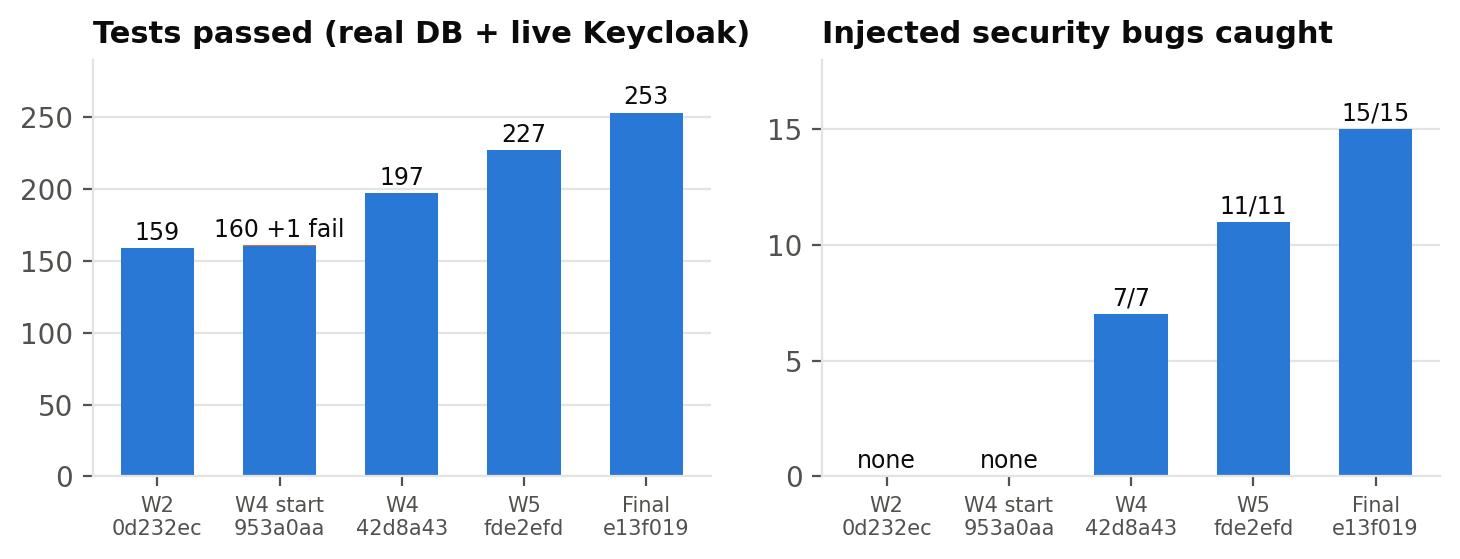
\includegraphics[width=0.53\textwidth]{verification-over-revisions.png}\hfill
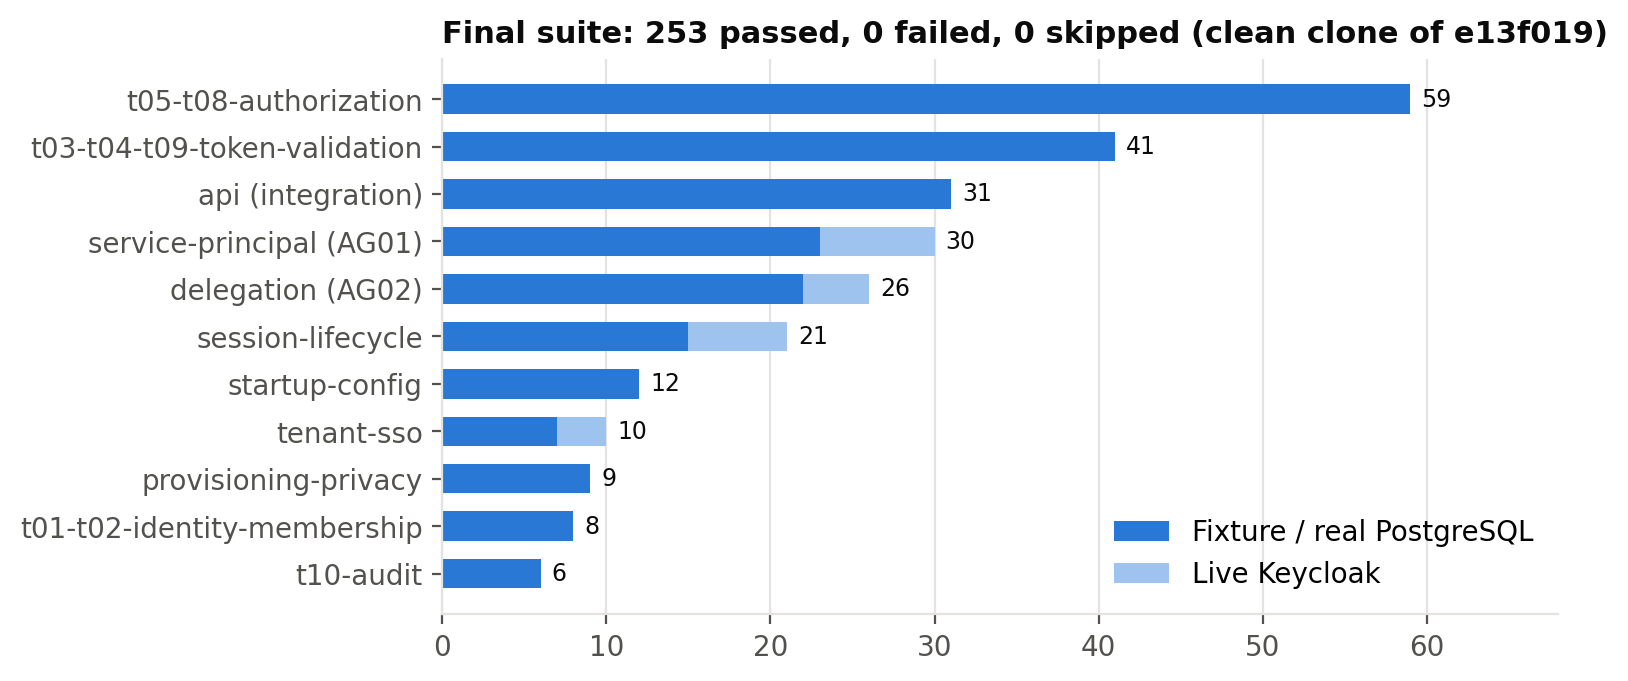
\includegraphics[width=0.45\textwidth]{final-suite-by-file.png}
\caption{Left: verification at each verified revision. The revision baseline \texttt{953a0aa} (160 passed, 1 failed, 6 skipped) exposed a real regression. Right: the final suite by file (light = live provider).}
\end{figure}

\textbf{Critical edge and failure cases covered.} Cross-tenant ID $\rightarrow$ 404. \code{X-Organization-ID} substitution $\rightarrow$ no data. A suspended member $\rightarrow$ 403, but may still withdraw consent. Provider outage $\rightarrow$ 503, not 401. Unsafe configuration $\rightarrow$ the process refuses to start. Refresh-token replay $\rightarrow$ the whole token family is revoked. Password reset alone $\rightarrow$ the session survives (documented). 12 concurrent first logins $\rightarrow$ one user. ID token used as an API credential $\rightarrow$ 401. An audit insert failure $\rightarrow$ the change is rolled back.

\section{Mutation testing: can the tests fail? (Q2)}
\begin{longtable}{@{}l P{9.6cm} c r@{}}
\toprule
\textbf{ID} & \textbf{Security guard removed on purpose} & \textbf{Added} & \textbf{Result}\\
\midrule
\endhead
M1 & Tenant membership check in \code{tenantContextHook} & W4 & killed (4)\\
M2 & JWT signature verification & W4 & killed (9)\\
M3 & Tenant filter on the submission lookup & W4 & killed (1)\\
M4 & Consent route admits suspended members for withdrawal & W4 & killed (4)\\
M5 & Fatal security-configuration check before \code{listen()} & W4 & killed (1)\\
M6 & Provider outage reported as 503, not as a bad credential & W4 & killed (6)\\
M7 & Casbin explicit-deny precedence & W4 & killed (3)\\
M8 & Service-principal registry refuses a disabled principal & W5 & killed (1)\\
M9 & Service token bound to its client's service account & W5 & killed (1)\\
M10 & Human-only routes refuse service principals & W5 & killed (3)\\
M11 & Service grant must match the exact action & W5 & killed (1)\\
M12 & Delegated agent needs the exact delegated scope & Final & killed (2)\\
M13 & Delegated agent is also limited by the user's permission & Final & killed (3)\\
M14 & A revoked delegation is refused & Final & killed (1)\\
M15 & Only delegable agents can receive a delegation & Final & killed (1)\\
\midrule
--- & Control: database container stopped & --- & \textsc{inconclusive}, exit 2\\
\bottomrule
\caption{Mutation results, clean clone of \texttt{e13f019}, 14 Nov 2026 (number of failing tests in brackets). Baseline before mutating: 233 passed, 0 failed, 20 skipped (live cases skip by design). Working tree unchanged afterwards.}
\end{longtable}

\section{Real-browser proof (Q5) and AG02 outcomes (Q6)}
\textbf{Browser proof} (\gh{scripts/verify-pkce.mjs}{\code{scripts/verify-pkce.mjs}}, Microsoft Edge): \textbf{11/11} on \code{localhost} and \textbf{11/11} on \code{127.0.0.1} with no source change (14 Nov). The checks: (1) the provider-admin service account cannot change realm settings; (2) a wrong PKCE verifier is rejected; (3) web login with S256 PKCE and signed audience/type/subject checks; (4) the same user is admin in one tenant and learner in the other, members 403, cross-tenant ID 404, tenant-scoped audit; (5) an AG02 delegation created in the browser is used by the real agent (200 in scope, 403 on members and in the other tenant, 401 after revocation); (6) mobile-client login; (7--8) enterprise broker login on web and mobile; (9) own-session listing excludes other users; (10) refresh rotation and replay rejection; (11) revoking one session rejects its tokens while another device stays signed in.

\begin{table}[H]
\centering\small
\begin{tabularx}{\textwidth}{@{}L L@{}}
\toprule
\textbf{AG02 property (Week~1 design)} & \textbf{Observed (26 tests, 4 live)}\\
\midrule
Agent with no delegation & 403\\
Within the delegated scope & 200; only published resources and only the delegator's own submissions\\
Scope delegated, but the user lacks the permission & 403; grade unchanged\\
User has the permission, but it was not delegated & human 200, agent 403\\
Teaching relationship & taught course 200, untaught course 403\\
Delegation used in another tenant & 403\\
Administrative scopes & 400 \code{SCOPE\_NOT\_DELEGABLE}; admin's agent 403 on six admin routes\\
Revocation / expiry / role loss / suspension / disabled agent & 401 (first request, 17 ms) / 401 / 403 / 403 / 401\\
Re-delegation by an agent; human sending a delegation header & 403 \code{PRINCIPAL\_KIND\_NOT\_ALLOWED}; 400\\
\bottomrule
\end{tabularx}
\caption{AG02 results: effective permission = user's current permission $\cap$ delegated scope $\cap$ tenant.}
\end{table}

\section{Cost of the per-request check (Q4)}
\begin{minipage}[t]{0.46\textwidth}\vspace{0pt}\small
\begin{tabular}{@{}lcc@{}}
\toprule
\textbf{Series} & \textbf{p50 (ms)} & \textbf{p95 (ms)}\\
\midrule
B0 local JWT verify & 0.15 & 0.28\\
\code{GET /health} (no auth) & 0.65 & 1.54\\
Introspection alone & 3.29 & 5.58\\
Full agent request (ours) & 9.25 & 15.14\\
\bottomrule
\end{tabular}\\[5pt]
Median of 3 runs $\times$ 200 sequential requests inside the backend container, 14 Nov (\gh{docs/evidence/2026-11-14/latency.log}{\code{latency.log}}); B0 from 500 local verifications on 16 Nov. The 16 Nov clean clone measured 2.11\,ms for introspection and 5.92\,ms for the agent request (p50). These are single-machine observations, not a benchmark; nothing was optimised and introspection was never disabled.
\end{minipage}\hfill
\begin{minipage}[t]{0.51\textwidth}\vspace{0pt}
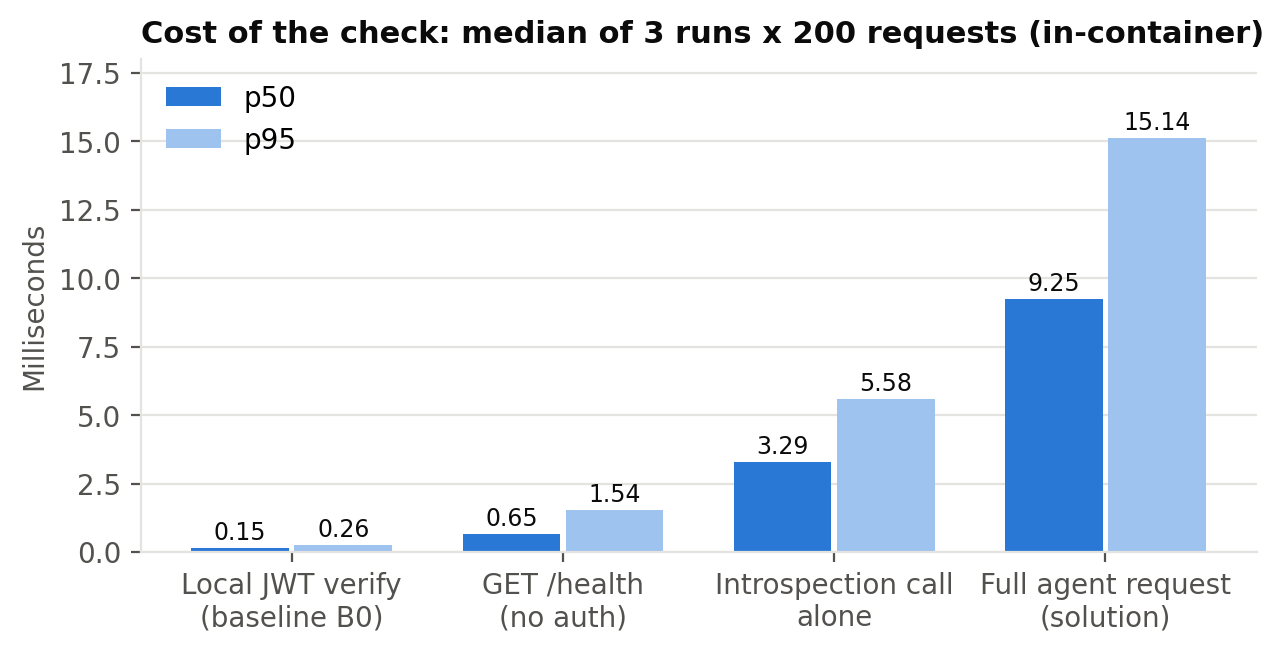
\includegraphics[width=\textwidth]{latency-cost.png}
\end{minipage}

\textbf{Revocation latency over time} (operation $\rightarrow$ first 401, ms): provider logout 62 / 62 / 45 / 64; own-session revocation 65 / 52 / 41 / 60; admin logout-all 38 / 31 / 26 / 33 (2 Oct / 31 Oct / 7 Nov / 14 Nov). AG01 disable: 23 (7 Nov), 29 (14 Nov). AG02 revoke: 17 (14 Nov). The test bound is 5000\,ms.

\section{Conclusions and limitations of the evaluation}
\textbf{Conclusions supported by the evidence.} (1) Every frozen acceptance criterion is met on a clean clone of the final revision. (2) Every one of the 15 security guards, when removed, is caught by named tests, so the suite is not vacuous. (3) Compared with the JWT-only baseline, uncached introspection turns ``valid until expiry'' (up to 60\,s for agents, 300\,s for users) into refusal on the very next request, at a measured cost of about 2--3\,ms per request.

\textbf{Tests not run (disclosed).} There was no independent rerun on a second machine (GitHub issue \#1). There was no concurrency or throughput load test (issue \#9). iOS/Safari were not tested. The physical-phone run (Android Chrome, 7 Nov) predates AG02. The 16 Nov clean-clone run completed steps 1--5 (stack, checks, 253/253 tests, E1, latency); its browser-proof and mutation steps did not complete because the host ran low on memory, so the evidence for those two checks is the 14 Nov clean run of identical code.

\section{Raw results and how to reproduce}
\begin{table}[H]
\centering\small
\begin{tabularx}{\textwidth}{@{}P{5.6cm} L@{}}
\toprule
E1 raw trials, summary, figures & \ghtree{evaluation/results/2026-11-16}{\code{evaluation/results/2026-11-16/}}\\
16 Nov fresh-clone logs & \ghtree{evaluation/results/2026-11-16-clean}{\code{evaluation/results/2026-11-16-clean/}}\\
14 Nov final clean run (suite, mutations, browser, latency) & \ghtree{docs/evidence/2026-11-14}{\code{docs/evidence/2026-11-14/}}\\
Dated evidence log for all revisions & \gh{docs/verification-evidence.md}{\code{docs/verification-evidence.md}}\\
Evaluation README (questions, baselines, commands) & \gh{evaluation/README.md}{\code{evaluation/README.md}}\\
\bottomrule
\end{tabularx}
\end{table}
\begin{scriptsize}
\begin{verbatim}
docker compose up -d --build --wait
# full suite (gated live provider tests)
$env:IAM_ALLOW_PASSWORD_GRANT_TESTS = "true"
node scripts/configure-keycloak.mjs --enable-test-client
docker compose exec -T backend env KEYCLOAK_INTROSPECTION=false RUN_DATABASE_TESTS=1 RUN_KEYCLOAK_TESTS=1 npm test
# E1 baseline vs solution (about 6 minutes)
Get-Content evaluation/scripts/baseline-revocation.mjs | docker compose exec -T backend node --input-type=module -
node scripts/configure-keycloak.mjs
Remove-Item Env:IAM_ALLOW_PASSWORD_GRANT_TESTS
node scripts/verify-test-independence.mjs        # mutations: exit 0 only if all killed
node scripts/verify-pkce.mjs                      # browser proof: 11 PASS lines
python evaluation/scripts/make_figures.py evaluation/results/<date>
# or everything from a fresh clone:
$s = "evaluation\run-clean-evaluation.ps1"
powershell -ExecutionPolicy Bypass -File $s -Revision cs5903-final-2026 -BrowserChannel msedge
\end{verbatim}
\end{scriptsize}
\end{document}
